\section{相关技术及背景}

\subsection{建筑工程图的认识}
建筑工程图是用来表示房屋的规划位置、外部造型、内部布置、内外装修、细致结构、固定设施及施工要求等的图纸。它包括施工图平面图、建筑总平面图、建筑剖面图、建筑立面图和建筑详图。

工程图纸分类分为三种:建筑施工图(又称建施),主要表示房屋的总平面图、剖面图、立面图等;结构施工图(又称结施),主要表示房屋承重结构的布置、构件类型、大小、数量及做法等。它包括结构布置图和构件详图;设施施工图(又称设施),主要表示各种线路、设备和管道的布置、走向以及安装施工要求等。

而本课题采用的建筑工程图属于建筑施工图的房屋平面图(文章以下出现的“工程图”时均表示建筑平面图)。而在现今,国内建筑行业在绘制平面图普遍使用AutoCAD软件绘制成.dwg文件格式的工程图。

.dwg是AutoCAD软件保存图形及属性数据的一种二进制文件格式,是制图行业的工业标准,数据结构复杂,主要包括文件头部(HEADER)、应急头部(CON-TINGENY HEADER)、表部(TABLES)、实体部(ENTITLES)、块实体部(BLOCKS)5部分。


\subsection{OpenCV的基础知识}
\subsubsection{OpenCV介绍}
OpenCV(Open Source Computer Vision Library)诞生于Intel研究中心,其目的是开发开一个普遍可用的计算机视觉库。在Inter的性能库团队的帮助下,OpenCV实现了一些关于计算机视觉的核心代码以及算法,并在Inter俄罗斯的库团队的帮助下得到优化。

OpenCV是一个开源的是计算机计算机视觉库。OpenCV采用 C/C++语言编写,可以运行在Linux/Windows/Mac等操作系统上。OpenCV还提供了可Python、Ruby、MATLAB以及其他语言的接口。无论是科研使用还是商业使用,OpenCV都是开放源代码且免费的,OpenCV的代码可用于或者嵌入(整体或部分)其他的应用程序中。

OpenCV主体分为五个模块,其中四个模块如图1所示。还有一个模块是CvAux模块,该模块中一般存放一些新出现的实验性的算法和函数,同时还有一些即将被淘汰的算法和函数。
\begin{figure}[htbp]
    % caption放上面就会显示在图的上方,出现在下面就是出现在图的下方
    \label{gra1}
    \begin{center}
        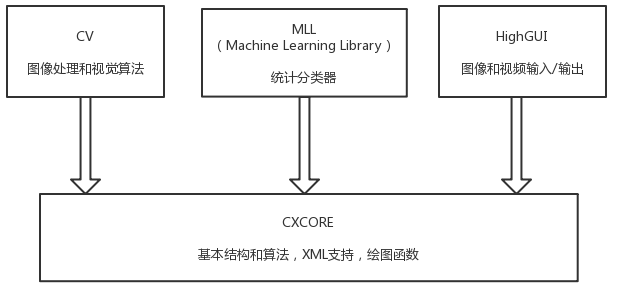
\includegraphics[width=3.6in]{OpenCV_module}
        \caption{OpenCV模块图}
    \end{center}
\end{figure}

\subsubsection{灰度处理}
% \begin{spacing}
% \subsubsubsection{灰度的概念:}
% ----------
灰度的概念:
% \end{spacing}

一个大小为$M * N$的数字图像是由$M$行$N$列的有限元素组成的,每个元素(又称为像素)都有特定的位置和幅值,代表了所在行列位置上的图像物理信息,如灰度和RBG等。

在二指图像(像素只有0和1两种取值,0代表黑色,1代表白色)中进一步加入许多介于黑色和白色之间的颜色深度,就构成了灰度图像。这类图像通常显示为从最暗黑色到最亮的白色的灰度,每种灰度(颜色深度)称为一个灰度级,通常用L表示。在灰度图像中,像素可以取0~L-1
之间的整数值,根据保存灰度数值所使用的数据类型不同,可能有256种取值或者$2^k$种取值,当k=1时即退化为二指图像。在通常情况下,图像的灰度级范围从0到255,白色为255,黑色为0,故黑白图片又称为灰度图像。灰度级越大表示越亮。

% ----------
图像灰度级分辨率:

在数字图像处理中,灰度级分辨率又称色阶,是指图像中可分辨的灰度级数目$L$,
它与存储灰度级别所使用的数据类型有关。由于灰度级度量的是投射到传感器上光辐射
值的强度,所以灰度级分辨率也叫辐射计量分辨率。

随着图像的灰度级分辨率逐渐降低,图像中包含的颜色数目变少,从而在颜色的角
度造成图像信息受损,同样使图像细节表达受到了一定的影响。

% ----------
灰度图像在图像处理中的作用:

对于一个数字图像处理系统来说,一般可以将处理流程分为3个阶段。在获取原始图像后,首先是图像预处理阶段,第二是特征抽取阶段,最后才是识别分析阶段。预处理阶段尤为重要,这个阶段处理不好则后面的工作根本无法展开。

灰度直方图是最基本的图像分析工具。灰度直方图是图像的一种统计表达,它反映了该图中不同灰度级出现的统计概率。主要应用于图像分割和图像灰度变换等处理过程中。

利用直方图辅助实现的各种灰度变换(点运算)\footnote{点运算:是指对一副图像中每个像素点的灰度值进行计算的方法。}
,包括线性灰度变换、分段线性灰度变换、非线性灰度变换等。

% ----------
阈值处理:

根据用户规定的阈值(threshold),一张图像每个像素的灰度值放在一个数组中,然后根据数值中的每个元素的值低于还是高于阈值而进行一些处理。例如阈值的二值化处理,图像中每个像素点的灰度值如果大于threshold,则这个值置为255;如果小于threshold,则将这个值置为0。

% ----------
直方图均衡化:

把原始图像的直方图变换为均匀分布的形式,从而增加图像灰度的动态范围,达到增强图像对比度的效果。经过均衡化的图像,其灰度级出现的概率相同,此时图像的熵\footnote{熵指的是体系的混乱的程度,对焦良好的图像的熵大于没有清晰对焦的图像,因此可以用熵作为一种对焦评价标准。熵越大,图像越清晰。——来源百度百科}
最大,图像所包含的信息量最大。

\begin{figure}[htbp]
    % caption放上面就会显示在图的上方,出现在下面就是出现在图的下方
    \label{gra1}
    \begin{center}
        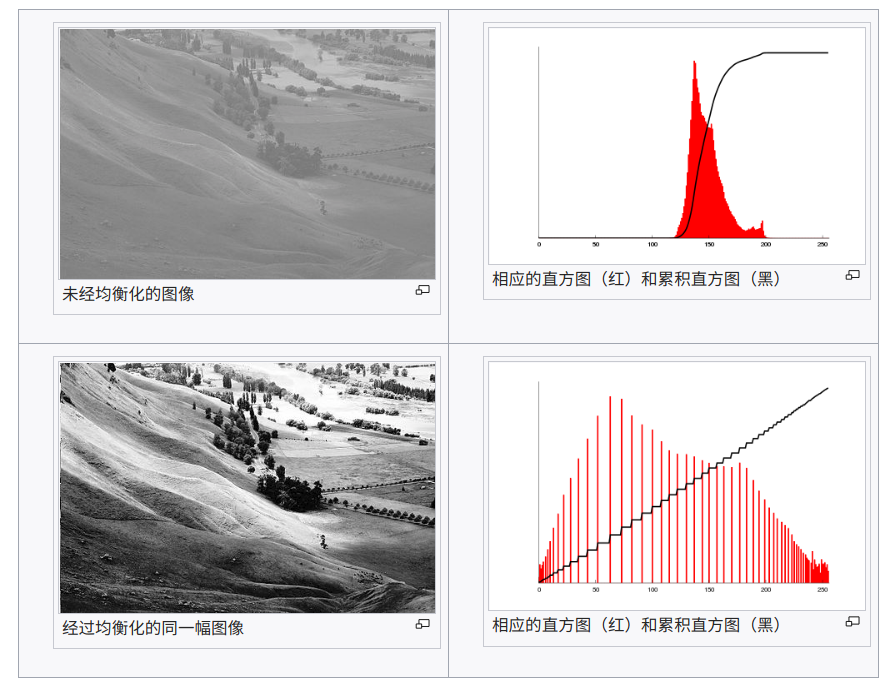
\includegraphics[width=3.6in]{Histogram_equalization}
        \caption{直方图均衡化前后对比}
    \end{center}
\end{figure}


\subsubsection{图像分割}

% -------------
图像分割概述:

图像分割是指将图像中具有特殊意义的不同区域划分出来,这些区域是互不相交的, 每个区域满足灰度、纹理、彩色等特征的某种相似性准则。

图像分割算法一般基于图像灰度值的两个基本特性之一:不连续性和相似性。第1类是基于图像灰度的不连续变化分割图像,例如图像的边缘,有边缘检测、边界跟踪、Hough变换等算法。第2类是依据事先制定的准则将图像分割为相似的区域,如阈值分割。

% ---------
图像分割的作用:

图像分割是图像识别和图像理解的前提步骤,图像分割质量的好坏直接影响了后续图像处理的效果。

\begin{figure}[htbp]
    % caption放上面就会显示在图的上方,出现在下面就是出现在图的下方
    \label{gra1}
    \begin{center}
        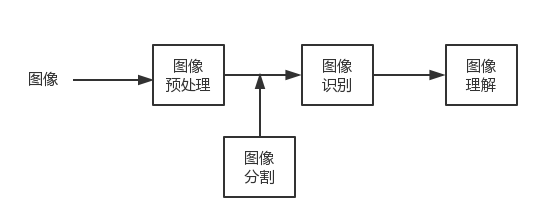
\includegraphics[width=4in]{Image_Segmentation.png}
        \caption{直方图均衡化前后对比}
    \end{center}
\end{figure}


% ----------
图像分割应用:

在交通上,应用于车辆检测、车辆跟踪、车种识别等;在生物医学上,应用于计算机断层图像CT、核磁共振、X光透视、病毒细胞的自动检测和识别等;在工业上,应用于产品的精度和纯度分析、矿藏分析、无接触式检测等;另外,在神经网络、机器人视觉、图像传输、身份鉴定等都各个领域都有着广泛的应用。


% ----------
Canny算法的步骤:

Canny边缘检测的基本思想就是首先对图像选择一定的Gauss(高斯)滤波器进行平滑滤波,然后采用非极值抑制技术进行处理得到最后的边缘图像。步骤如下:

(1)用高斯滤波器平滑图像
滤波的主要目的是降噪,高斯滤波会将图像变得模糊,同时也会可能增加边
缘的宽度。对于在图像中位置$(m,n)$的像素点,其灰度值为$f(m,n)$。

\bf{$g_{\sigma}(m,n) = \frac{1}{\sqrt{2\pi\sigma^2}} e^{\frac{-m^2+n^2}{2{\sigma^2}}} \cdot f(m,n) $}


$H_x = \begin{bmatrix} -1 & -2 & -1 \\ 0 & 0 & 0  \\ 1 & 2 & 1\end{bmatrix}$ \quad{}
$H_y = \begin{bmatrix} -1 & 0 & 1 \\ -2 & 0 & 2  \\ -1 & 0 & 1\end{bmatrix}$

$ G_x = H_y \cdot f(m,n)$ \quad{} $ G_y = H_x \cdot f(m,n)$


$G(m,n) = \sqrt{G_x(m,n) ^2 + G_y(m,n)^2}$

$\theta = arctan \frac{G_x(m,n)}{G_y(m,n)} $

\quad{}

$\rho = xcos \theta +ysin \theta$

\quad{}

$T_{TOF} =[(Ta_1 - Ta_2) - (Tb_1 - Tb_2)] /2 $ \quad{}\quad{}(1)

\quad{}

$ S= C \cdot T_{TOF}$ , \quad{}(C为光速, 即 $C=3\cdot 10^8$ ) \quad{}\quad{}(2)

\quad{}

$d_i^2 = (x - x_i)^2 + (y - y_i)^2 $ \quad{}\quad{}(1)

\quad$ = x^2 -2x_ix + x_i^2 + y^2 - 2y_iy + y_i^2$ , \quad{}其中$(i = 0,1,2)$

\quad

$d_i^2 - d_N^2 = -2x(x_i - x_N) + x_i^2 -x_N^2 $ \quad{}\quad{}(2)

\quad\quad\quad\quad{} $- 2y(y_i-y_N) + y_i^2 - y_N^2$, \quad{}其中$(i = 0,1,2\dots, N-1)$

\quad{}

$b = \begin{bmatrix} d_0^2 - d_2^2 - (x_0^2 + y_0^2) + (x_2^2 + y_2^2) \\ d_1^2 - d_2^2 - (x_1^2 + y_1^2) + (x_2^2 + y_2^2) \end{bmatrix}$ \quad{}\quad{}(3)

\quad

$A = -2 \begin{bmatrix} x_0 - x_2 & y_0 - y_2 \\ x_1 - x_2 & y_1 - y_2 \end{bmatrix}$ \quad{}\quad{}(4)

\quad

$X = A^{-1}b$ \quad\quad(5)求解

\quad{}

$G_T(m,n) = \begin{cases}
    G(m,n), & if\quad{} G(m,n)>=T \\
    0, & $其他情况$
    
\end{cases} $

\[ y=\begin{cases}
    -x & x<0\\
    x & x\geq0
    \end{cases} \]
    

\quad

$PPI = \sqrt{1920^2 + 1080^2}/15.6 = 141.21$

\quad

$DP = 15.* 25.4 / \sqrt{1920^2 + 1080^2} = 0.1799$ ,(其中1英寸 = 25.4 mm)